% Desde la raíz del repositorio, incluir con:
% % Desde la raíz del repositorio, incluir con:
% % Desde la raíz del repositorio, incluir con:
% % Desde la raíz del repositorio, incluir con:
% \input{FORM-AC-01 - Análisis de caso - Fallo en sistema distribuido real - Loor Mendoza Byron Daniel/causas-raiz.tex}
% En el preámbulo, cargar las entradas con:
% \addbibresource{FORM-AC-01 - Análisis de caso - Fallo en sistema distribuido real - Loor Mendoza Byron Daniel/referencias.bib}
\section{Causas raíz}

El 2 de junio de 2019, a las 11:45 PDT, comenzó un mantenimiento en una sola ubicación física. En las regiones afectadas, los procesos del plano de control de red y su infraestructura de soporte estaban configurados para detenerse durante el mantenimiento. Varias instancias del gestor de clústeres que ejecutaban esos procesos podían quedar incluidas en ese tipo de mantenimiento. Un error en la automatización permitió detener varios clústeres independientes a la vez, incluso en ubicaciones físicas distintas. La red siguió funcionando unos minutos hasta que se retiraron rutas BGP entre los sitios afectados y cayó la capacidad de la red \cite{googlecloud19009}. Desde fuera de Google, ThousandEyes observó pérdida de paquetes en el borde de la red en las rutas que monitoreó \cite[fig.~4]{medina2019googlecloud}.

\begin{figure}[htbp]
  \centering
  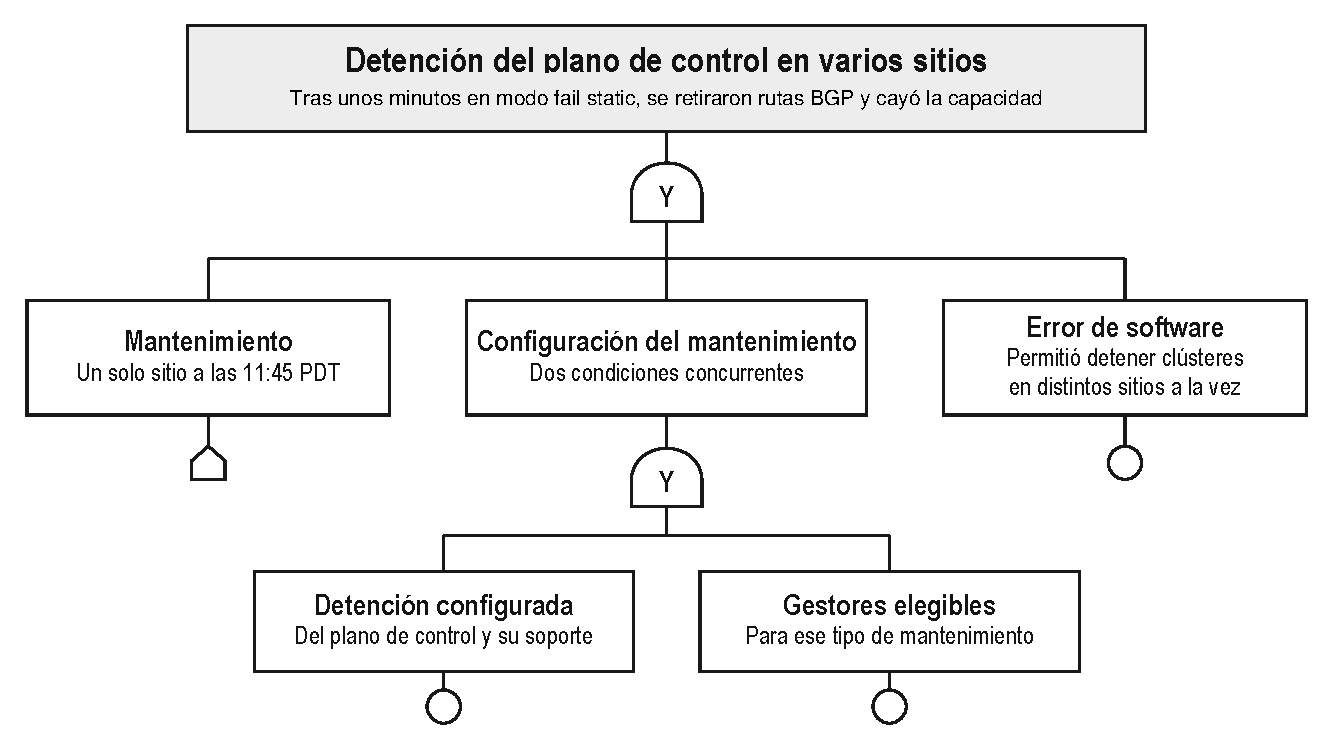
\includegraphics[width=0.88\linewidth]{diagrama-causas.pdf}
  \caption{Árbol de fallos del incidente de red. Elaborado a partir del informe de Google Cloud \cite{googlecloud19009}.}
  \label{fig:causas-google-cloud}
\end{figure}

\section{Lecciones aprendidas para CLAB}

CLAB, el proyecto de gestión de reservas de laboratorios de Byron, usa Angular, Spring Boot y PostgreSQL. A partir del caso de Google Cloud, se proponen tres medidas para TA-PFC-E1:

\begin{itemize}
  \item \textbf{Cambio de configuración.} Una actualización de la API podría cortar su conexión con PostgreSQL e impedir las reservas. Validaremos la consulta de disponibilidad y una reserva de prueba antes del despliegue, con una configuración anterior lista para revertir el cambio.
  \item \textbf{Reservas concurrentes.} Dos solicitudes simultáneas podrían encontrar libre el mismo laboratorio antes de guardar. Haremos que la base de datos rechace solapamientos concurrentes y probaremos dos solicitudes para el mismo horario.
  \item \textbf{Recuperación del servidor.} Si el diagnóstico depende del servidor afectado, una caída puede retrasar la recuperación. Comprobaremos la disponibilidad desde otro equipo y probaremos la restauración de copias de la configuración y de la base de datos guardadas fuera del servidor.
\end{itemize}

\paragraph*{Declaración de uso de inteligencia artificial}
Leí el informe de Google Cloud e identifiqué las dos configuraciones y el error de software que causaron el fallo. Usé OpenAI Codex (GPT-6.1 Sol, esfuerzo de razonamiento alto) para ajustar la redacción del literal B, preparar el árbol de fallos en draw.io y su PDF, cotejar las referencias e incorporar el apartado en LaTeX. Contrasté las causas con el informe oficial y revisé los rótulos y las conexiones del diagrama.

% En el preámbulo, cargar las entradas con:
% \addbibresource{FORM-AC-01 - Análisis de caso - Fallo en sistema distribuido real - Loor Mendoza Byron Daniel/referencias.bib}
\section{Causas raíz}

El 2 de junio de 2019, a las 11:45 PDT, comenzó un mantenimiento en una sola ubicación física. En las regiones afectadas, los procesos del plano de control de red y su infraestructura de soporte estaban configurados para detenerse durante el mantenimiento. Varias instancias del gestor de clústeres que ejecutaban esos procesos podían quedar incluidas en ese tipo de mantenimiento. Un error en la automatización permitió detener varios clústeres independientes a la vez, incluso en ubicaciones físicas distintas. La red siguió funcionando unos minutos hasta que se retiraron rutas BGP entre los sitios afectados y cayó la capacidad de la red \cite{googlecloud19009}. Desde fuera de Google, ThousandEyes observó pérdida de paquetes en el borde de la red en las rutas que monitoreó \cite[fig.~4]{medina2019googlecloud}.

\begin{figure}[htbp]
  \centering
  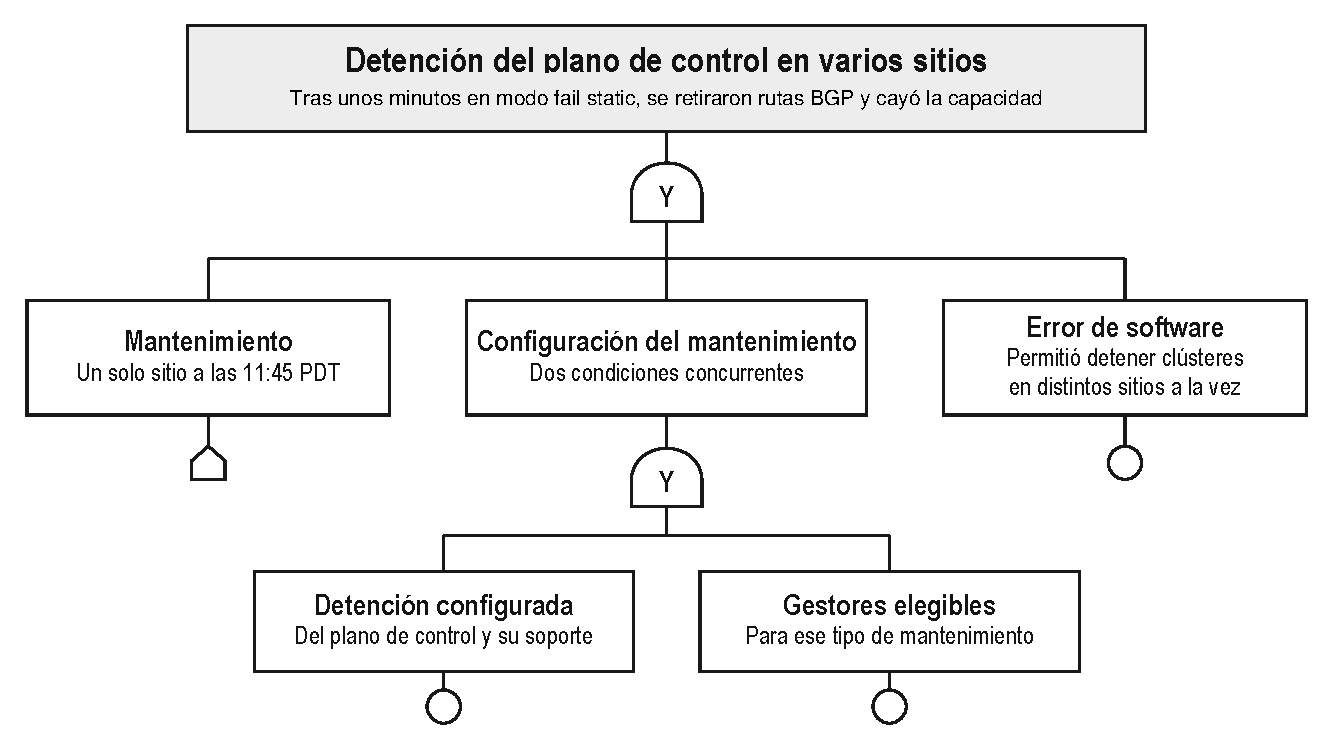
\includegraphics[width=0.88\linewidth]{diagrama-causas.pdf}
  \caption{Árbol de fallos del incidente de red. Elaborado a partir del informe de Google Cloud \cite{googlecloud19009}.}
  \label{fig:causas-google-cloud}
\end{figure}

\section{Lecciones aprendidas para CLAB}

CLAB, el proyecto de gestión de reservas de laboratorios de Byron, usa Angular, Spring Boot y PostgreSQL. A partir del caso de Google Cloud, se proponen tres medidas para TA-PFC-E1:

\begin{itemize}
  \item \textbf{Cambio de configuración.} Una actualización de la API podría cortar su conexión con PostgreSQL e impedir las reservas. Validaremos la consulta de disponibilidad y una reserva de prueba antes del despliegue, con una configuración anterior lista para revertir el cambio.
  \item \textbf{Reservas concurrentes.} Dos solicitudes simultáneas podrían encontrar libre el mismo laboratorio antes de guardar. Haremos que la base de datos rechace solapamientos concurrentes y probaremos dos solicitudes para el mismo horario.
  \item \textbf{Recuperación del servidor.} Si el diagnóstico depende del servidor afectado, una caída puede retrasar la recuperación. Comprobaremos la disponibilidad desde otro equipo y probaremos la restauración de copias de la configuración y de la base de datos guardadas fuera del servidor.
\end{itemize}

\paragraph*{Declaración de uso de inteligencia artificial}
Leí el informe de Google Cloud e identifiqué las dos configuraciones y el error de software que causaron el fallo. Usé OpenAI Codex (GPT-6.1 Sol, esfuerzo de razonamiento alto) para ajustar la redacción del literal B, preparar el árbol de fallos en draw.io y su PDF, cotejar las referencias e incorporar el apartado en LaTeX. Contrasté las causas con el informe oficial y revisé los rótulos y las conexiones del diagrama.

% En el preámbulo, cargar las entradas con:
% \addbibresource{FORM-AC-01 - Análisis de caso - Fallo en sistema distribuido real - Loor Mendoza Byron Daniel/referencias.bib}
\section{Causas raíz}

El 2 de junio de 2019, a las 11:45 PDT, comenzó un mantenimiento en una sola ubicación física. En las regiones afectadas, los procesos del plano de control de red y su infraestructura de soporte estaban configurados para detenerse durante el mantenimiento. Varias instancias del gestor de clústeres que ejecutaban esos procesos podían quedar incluidas en ese tipo de mantenimiento. Un error en la automatización permitió detener varios clústeres independientes a la vez, incluso en ubicaciones físicas distintas. La red siguió funcionando unos minutos hasta que se retiraron rutas BGP entre los sitios afectados y cayó la capacidad de la red \cite{googlecloud19009}. Desde fuera de Google, ThousandEyes observó pérdida de paquetes en el borde de la red en las rutas que monitoreó \cite[fig.~4]{medina2019googlecloud}.

\begin{figure}[htbp]
  \centering
  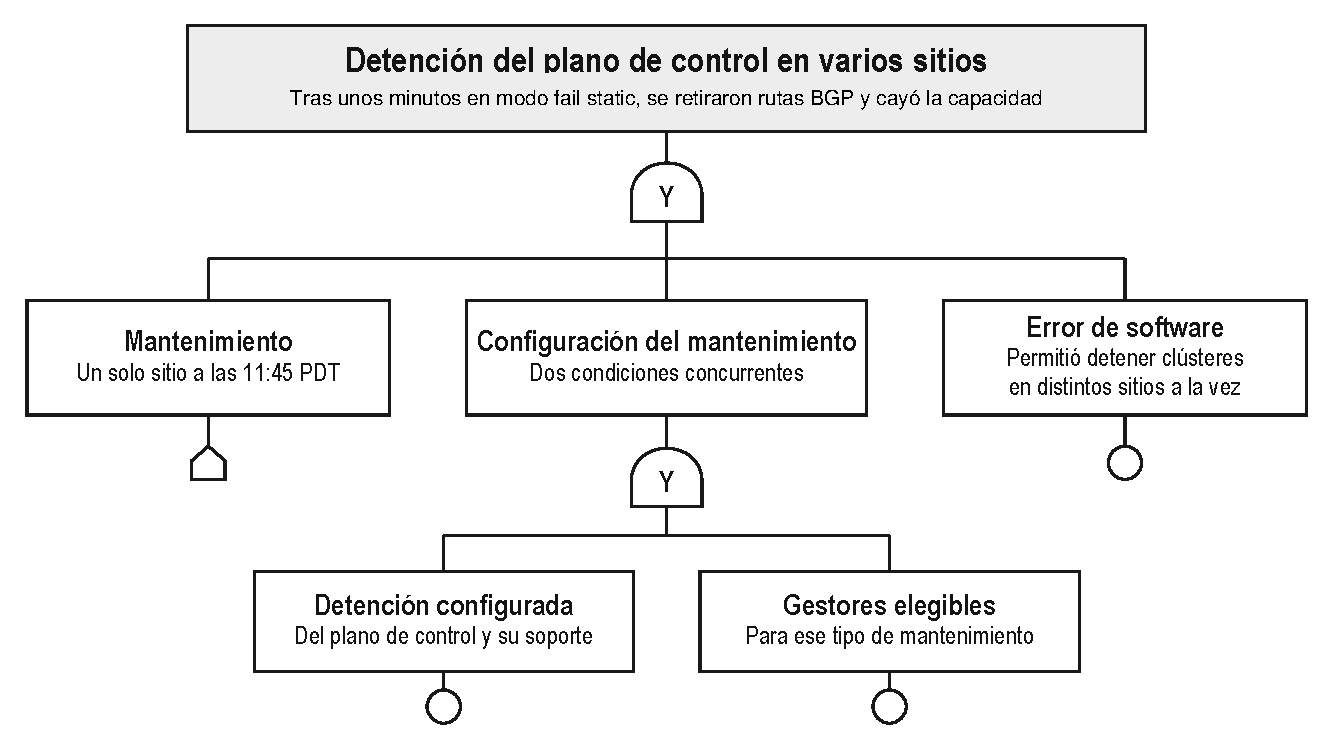
\includegraphics[width=0.88\linewidth]{diagrama-causas.pdf}
  \caption{Árbol de fallos del incidente de red. Elaborado a partir del informe de Google Cloud \cite{googlecloud19009}.}
  \label{fig:causas-google-cloud}
\end{figure}

\section{Lecciones aprendidas para CLAB}

CLAB, el proyecto de gestión de reservas de laboratorios de Byron, usa Angular, Spring Boot y PostgreSQL. A partir del caso de Google Cloud, se proponen tres medidas para TA-PFC-E1:

\begin{itemize}
  \item \textbf{Cambio de configuración.} Una actualización de la API podría cortar su conexión con PostgreSQL e impedir las reservas. Validaremos la consulta de disponibilidad y una reserva de prueba antes del despliegue, con una configuración anterior lista para revertir el cambio.
  \item \textbf{Reservas concurrentes.} Dos solicitudes simultáneas podrían encontrar libre el mismo laboratorio antes de guardar. Haremos que la base de datos rechace solapamientos concurrentes y probaremos dos solicitudes para el mismo horario.
  \item \textbf{Recuperación del servidor.} Si el diagnóstico depende del servidor afectado, una caída puede retrasar la recuperación. Comprobaremos la disponibilidad desde otro equipo y probaremos la restauración de copias de la configuración y de la base de datos guardadas fuera del servidor.
\end{itemize}

\paragraph*{Declaración de uso de inteligencia artificial}
Leí el informe de Google Cloud e identifiqué las dos configuraciones y el error de software que causaron el fallo. Usé OpenAI Codex (GPT-6.1 Sol, esfuerzo de razonamiento alto) para ajustar la redacción del literal B, preparar el árbol de fallos en draw.io y su PDF, cotejar las referencias e incorporar el apartado en LaTeX. Contrasté las causas con el informe oficial y revisé los rótulos y las conexiones del diagrama.

% En el preámbulo, cargar las entradas con:
% \addbibresource{FORM-AC-01 - Análisis de caso - Fallo en sistema distribuido real - Loor Mendoza Byron Daniel/referencias.bib}
\section{Causas raíz}

El 2 de junio de 2019, a las 11:45 PDT, comenzó un mantenimiento en una sola ubicación física. En las regiones afectadas, los procesos del plano de control de red y su infraestructura de soporte estaban configurados para detenerse durante el mantenimiento. Varias instancias del gestor de clústeres que ejecutaban esos procesos podían quedar incluidas en ese tipo de mantenimiento. Un error en la automatización permitió detener varios clústeres independientes a la vez, incluso en ubicaciones físicas distintas. La red siguió funcionando unos minutos hasta que se retiraron rutas BGP entre los sitios afectados y cayó la capacidad de la red \cite{googlecloud19009}. Desde fuera de Google, ThousandEyes observó pérdida de paquetes en el borde de la red en las rutas que monitoreó \cite[fig.~4]{medina2019googlecloud}.

\begin{figure}[htbp]
  \centering
  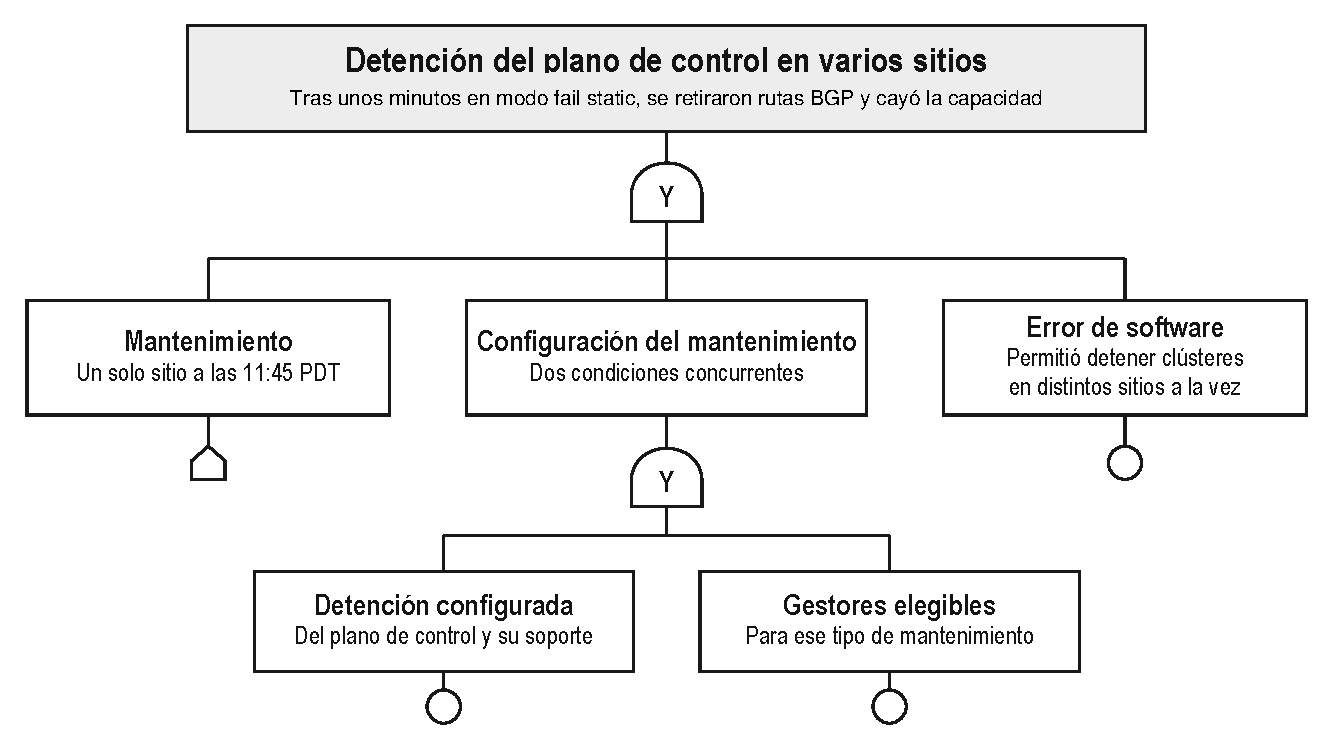
\includegraphics[width=0.88\linewidth]{diagrama-causas.pdf}
  \caption{Árbol de fallos del incidente de red. Elaborado a partir del informe de Google Cloud \cite{googlecloud19009}.}
  \label{fig:causas-google-cloud}
\end{figure}

\section{Lecciones aprendidas para CLAB}

CLAB, el proyecto de gestión de reservas de laboratorios de Byron, usa Angular, Spring Boot y PostgreSQL. A partir del caso de Google Cloud, se proponen tres medidas para TA-PFC-E1:

\begin{itemize}
  \item \textbf{Cambio de configuración.} Una actualización de la API podría cortar su conexión con PostgreSQL e impedir las reservas. Validaremos la consulta de disponibilidad y una reserva de prueba antes del despliegue, con una configuración anterior lista para revertir el cambio.
  \item \textbf{Reservas concurrentes.} Dos solicitudes simultáneas podrían encontrar libre el mismo laboratorio antes de guardar. Haremos que la base de datos rechace solapamientos concurrentes y probaremos dos solicitudes para el mismo horario.
  \item \textbf{Recuperación del servidor.} Si el diagnóstico depende del servidor afectado, una caída puede retrasar la recuperación. Comprobaremos la disponibilidad desde otro equipo y probaremos la restauración de copias de la configuración y de la base de datos guardadas fuera del servidor.
\end{itemize}

\paragraph*{Declaración de uso de inteligencia artificial}
Leí el informe de Google Cloud e identifiqué las dos configuraciones y el error de software que causaron el fallo. Usé OpenAI Codex (GPT-6.1 Sol, esfuerzo de razonamiento alto) para ajustar la redacción del literal B, preparar el árbol de fallos en draw.io y su PDF, cotejar las referencias e incorporar el apartado en LaTeX. Contrasté las causas con el informe oficial y revisé los rótulos y las conexiones del diagrama.
